\section*{Exercise 3}
\begin{enumerate}
	\item Make a figure to describe the architecture of your CNN. Specify the corresponding hyper-parameters and trainable parameters used in every layer of your network. Calculate manually the output size of each layer. 
	\item What is the total number of trainable parameters of your network? Report the results you get after certain number of epochs (e.g. 50) and compare them with the results obtained from VGGNet.

\end{enumerate}
For our 4-layer CNN, we chose 3 convolution layers followed by average pooling and a fully connected layer. As an activation function, we used ReLu and we added a dropout layer after the 3rd convolution layer. The figures below show the differences between the same CNN with the dropout layer and without. The final implementation can be found under \ref{CNN}.



\begin{figure}[htbp] 
    \centering
    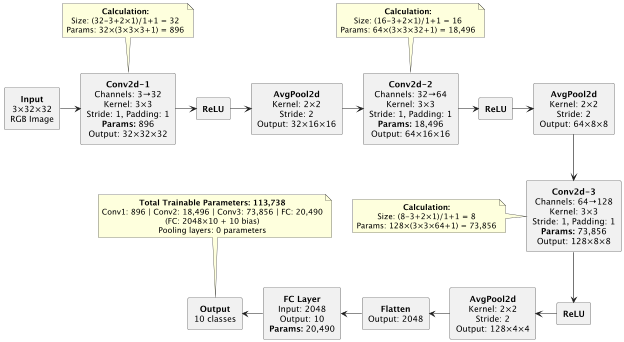
\includegraphics[width=1\textwidth]{images/ex3_architecture} 
    \caption{Custom cnn architecture}
\end{figure}

As displayed in the figure above, the total amount of trainable parameters is 113,738. The hyper-parameters are specified for each layer, namely the amount of channels, kernel size, stride and padding. Additional hyper-parameters are learning rate, batch size
number of epochs, loss function etc., however those remained untouched from the previous example of training VGGNet. The effect of a dropout layer, however, has been tested in detail with multiple runs of the CNN with and without it:

\begin{figure}[H]
    \centering
    \begin{subfigure}[t]{0.4\textwidth}
        \centering
        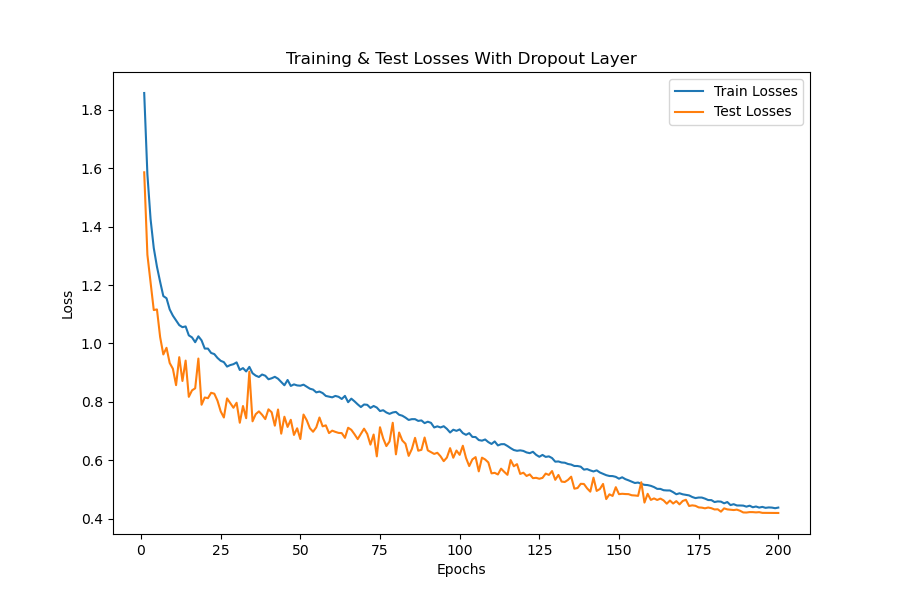
\includegraphics[width=\textwidth]{images/ex_3_Training & Test Losses With Dropout Layer.png}
        \caption{Average training vs. test loss with Dropout Layer.}
    \end{subfigure}
    \hfill
    \begin{subfigure}[t]{0.4\textwidth}
        \centering
        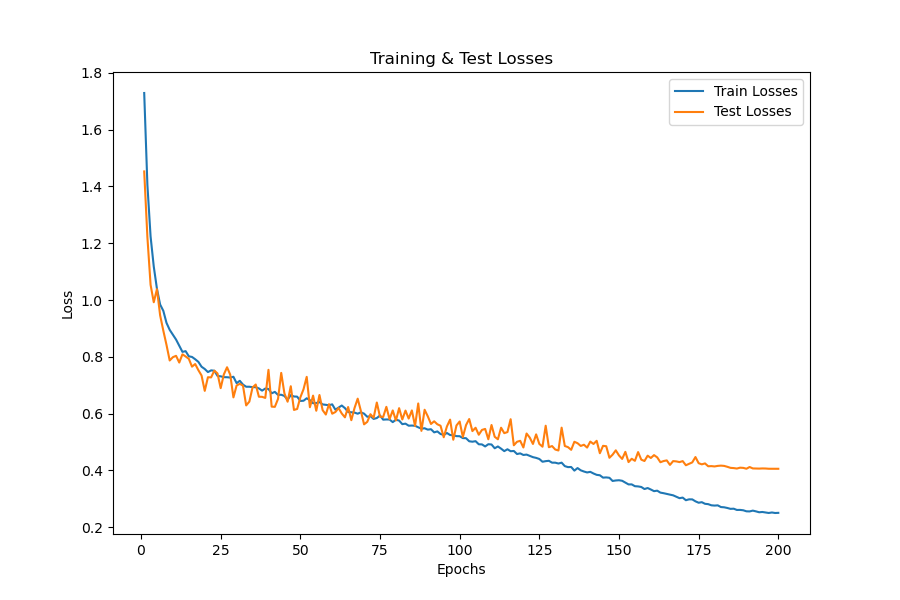
\includegraphics[width=\textwidth]{images/ex_3_Training & Test Losses.png}
        \caption{Average training vs. test loss without Dropout Layer.}
    \end{subfigure}
    \caption{Training vs. Test Loss with/out Dropout}
\end{figure}

\begin{figure}[H]
    \centering
    \begin{subfigure}[t]{0.4\textwidth}
        \centering
        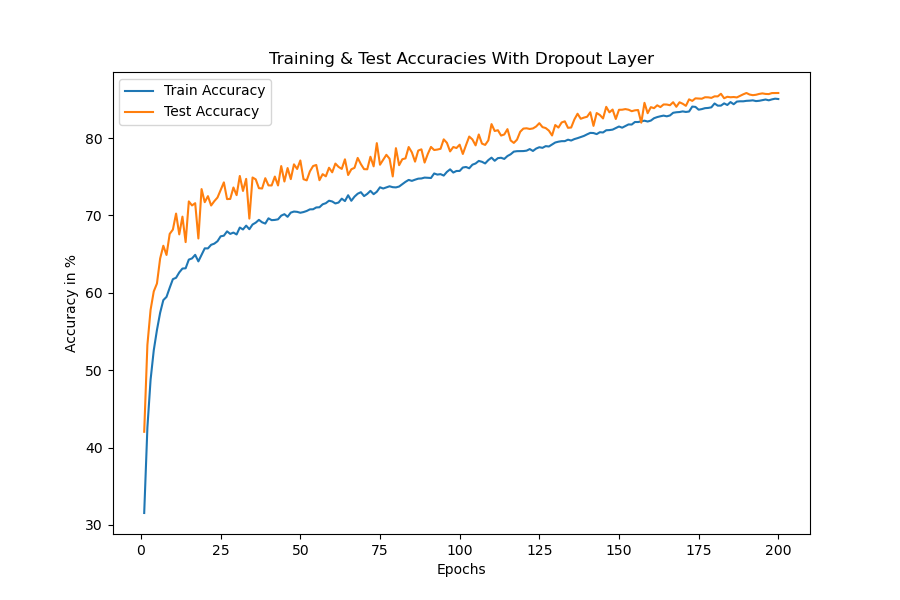
\includegraphics[width=\textwidth]{images/ex_3_Training & Test Accuracies With Dropout Layer.png}
        \caption{Average training vs. test accuracy with Dropout Layer.}
    \end{subfigure}
    \hfill
    \begin{subfigure}[t]{0.4\textwidth}
        \centering
        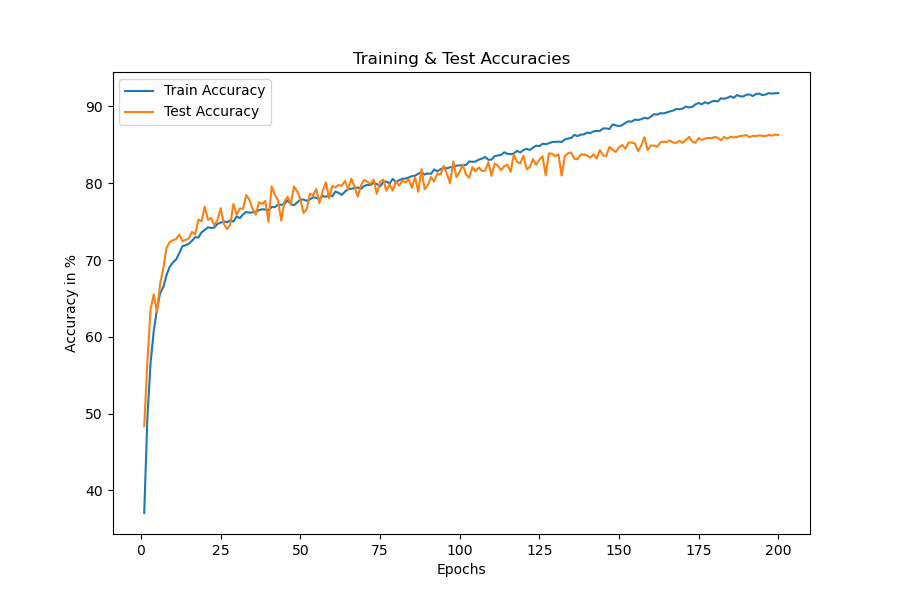
\includegraphics[width=\textwidth]{images/ex_3_Training & Test Accuracies.png}
        \caption{Average training vs. test accuracy without Dropout Layer.}
    \end{subfigure}
    \caption{Training vs. Test Accuracy with/out Dropout}
\end{figure}

\begin{figure}[H]
    \centering
    \begin{subfigure}[t]{0.48\textwidth}
        \centering
        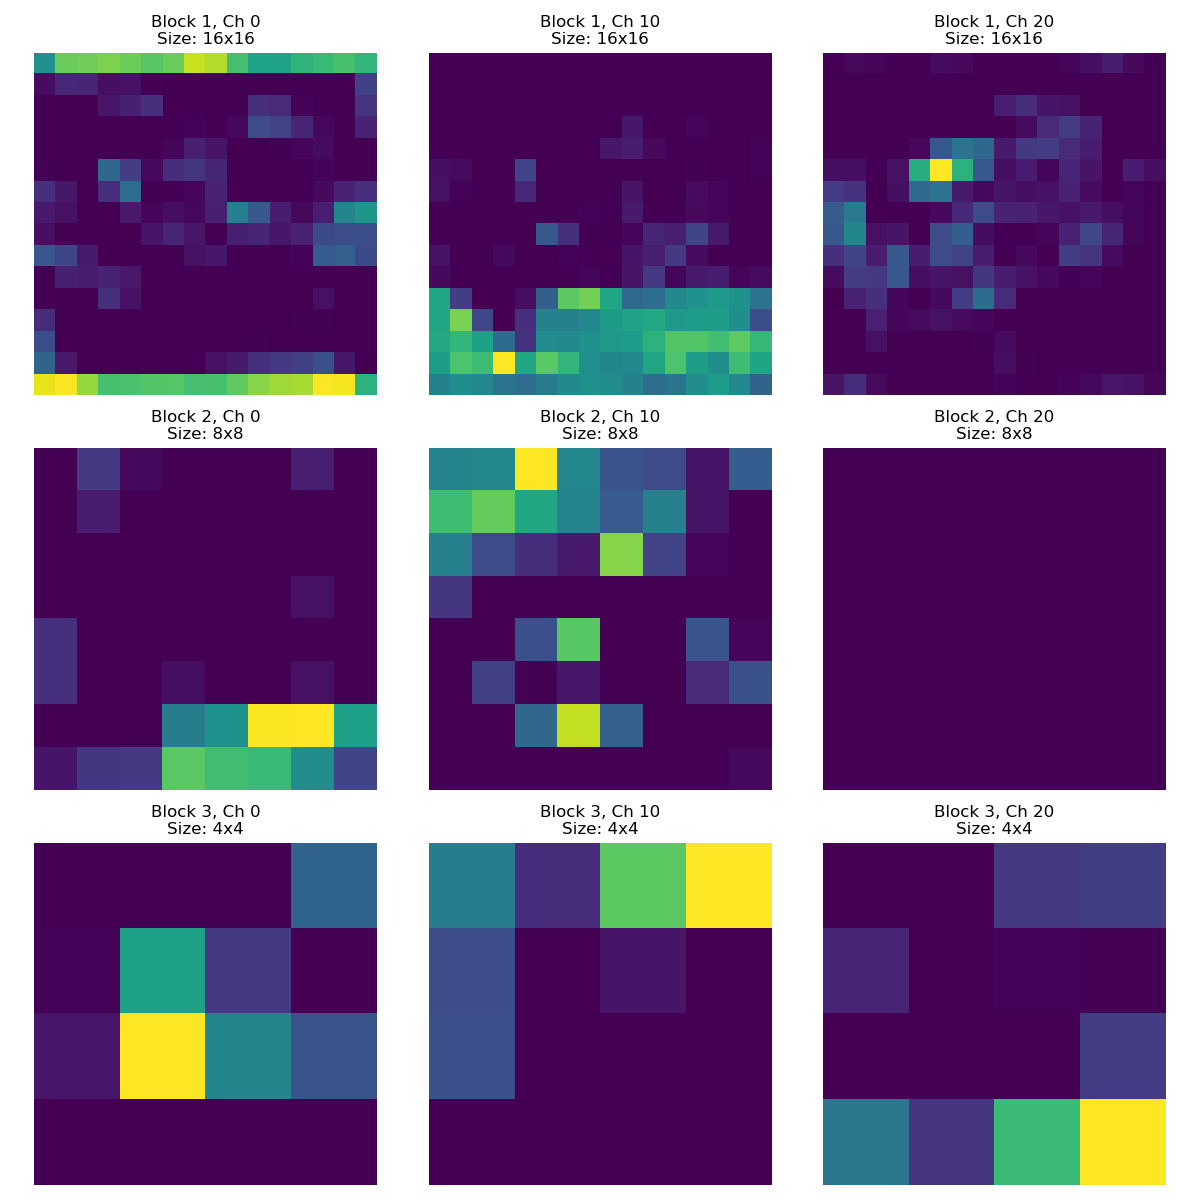
\includegraphics[width=\textwidth]{images/ex_3_feature_maps_visualization_dropout.png}
        \caption{Feature maps across 3 convolutional layers with Dropout Layer.}
    \end{subfigure}
    \hfill
    \begin{subfigure}[t]{0.48\textwidth}
        \centering
        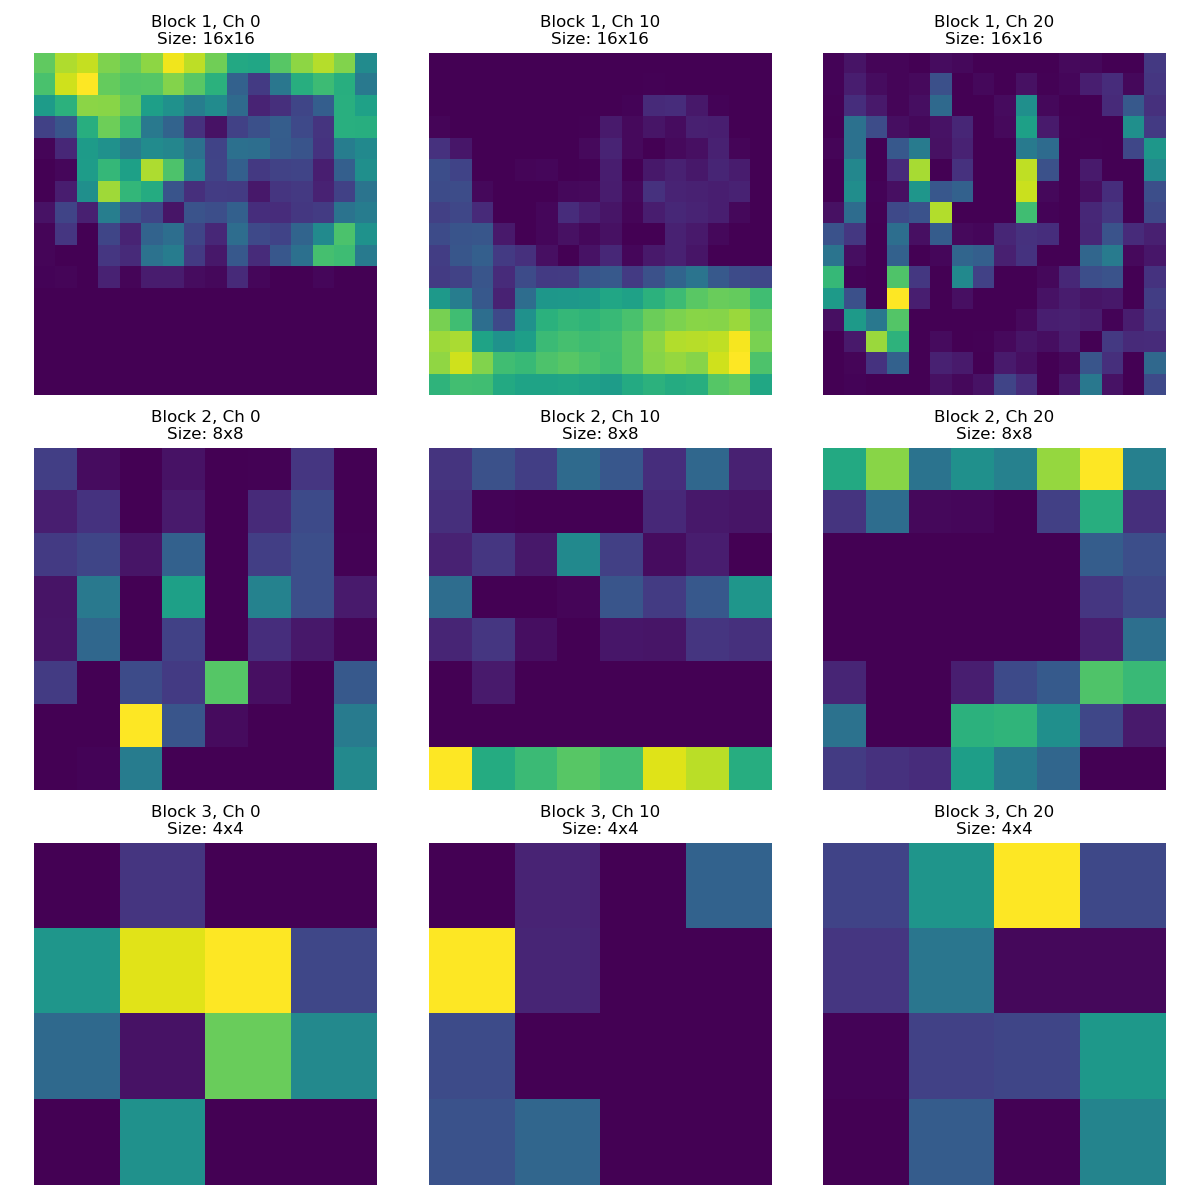
\includegraphics[width=\textwidth]{images/ex_3_feature_maps_visualization.png}
        \caption{Feature maps across 3 convolutional layers without Dropout Layer.}
    \end{subfigure}
    \caption{Feature maps across 3 convolutional layers with/out Dropout Layer.}
\end{figure}

\textbf{Loss}\\
The CNN with the dropout layer shows that the training and test losses are close, reducing overfitting. The CNN model without dropout creates a gap between the training and testing showing a poor generalization of data.

\textbf{Accuracy}\\
The CNN with the dropout layer shows less overfitting as the training and test accuracy curves remain closer throughout the training process, leading to a much smoother increase in test accuracy. The CNN model without dropout shows a clea sign of overfitting after aprox. 100 epochs where training accuracy continues to increase, but test accuracy plateaus significantly lower.

\textbf{Feature Maps}\\
The main difference between the feature maps is that the dropout layer propagates back through the network changing the final weight values of all previous layers.\\

\subsection*{Conclusion \& Comparison to VGG}
Based on the experimental comparison between the custom CNN with dropout and the VGG network on CIFAR-10, both architectures achieve approximately 90\% test accuracy after 200 epochs (with the custom CNN at ca. 75\% test accuracy and the VGG at ca. 82\% after 50 epochs respectively), yet the superior efficiency of the smaller network (113K parameters) demonstrates the importance of architecture-dataset alignment. The custom CNN's design is inherently well-suited for CIFAR-10's 32×32 images. The inclusion of dropout (p=0.5) provides crucial regularisation that prevents overfitting, while VGG's architecture, originally designed for ImageNet's larger 224×224 images and 1000 classes, introduces unnecessary computational overhead for the simpler CIFAR-10 classification task. This mismatch means VGG requires significantly more parameters and computational resources to achieve the same 90\% accuracy that the custom network reaches with far fewer resources. However, the VGG seems do to better in the first 50 epochs than the custom CNN. The combination of appropriate model complexity, effective regularisation through dropout, and architecture designed for the target image size explains why the custom CNN achieves equivalent test accuracy to the more complex VGG network while being substantially more efficient in terms of parameters and computational requirements.





